\documentclass{svproc}
%
\usepackage{url}
\usepackage[colorlinks=true, urlcolor=blue, citecolor=black, linkcolor=black]{hyperref}
\def\UrlFont{\rmfamily}
\usepackage{graphicx}
\usepackage{booktabs}
\usepackage{amsmath,amssymb}
\usepackage{algorithm}
\usepackage{algorithmicx}
\usepackage{algpseudocode}
\usepackage{float}

\begin{document}
\mainmatter

\title{A Heterogeneous Fleet Approach to the Capacitated Multi-Depot Vehicle Routing Problem with Time Windows for Indian Cooperative Dairy}

\titlerunning{Heterogeneous MDVRP for Indian Cooperative Dairy}

\author{Raj Patil\inst{1}\thanks{These authors contributed equally to this work.} \and Kushagra Kushwah\inst{1}\thanks{These authors contributed equally to this work.} \and Anshul Agarwal\inst{1} \and Manish Kurhekar\inst{1}}

\authorrunning{Raj Patil et al.}

\tocauthor{Raj Patil, Kushagra Kushwah, Anshul Agarwal, Manish Kurhekar}

\institute{Department of Computer Science and Engineering, Visvesvaraya National Institute of Technology (VNIT), Nagpur 440010, Maharashtra, India\\
\email{rajpatil280906@gmail.com, kushagrasinghkushwah46@gmail.com,}\\
\email{anshulagarwal@cse.vnit.ac.in, manishkurhekar@cse.vnit.ac.in}}

\maketitle

\begin{abstract}
Milk collection in Indian cooperative dairies is a critical logistical challenge owing to the product's short shelf life, geographically dispersed collection centres, and strict temporal constraints. This work addresses the Multi-Depot Vehicle Routing Problem (MDVRP) within Perishable Food Supply Chain Management, where the time-sensitive nature of the product demands optimisation well beyond standard freight routing. Using Google OR-Tools, we implement a Capacitated Vehicle Routing Problem with Time Windows (CVRPTW) supporting a heterogeneous vehicle fleet. A central contribution is the integration of real-road geometry via the Open Source Routing Machine (OSRM) to ensure route feasibility across complex rural terrain. Guided Local Search (GLS) with node disjunctions is used to prioritise high-volume centres and maximise milk recovery within shift limits. A fixed 5-minute pumping service time per Village Collection Centre (VCC) is modelled as a conceptual time-window constraint; reported results use travel-time-only routing as an analytical baseline that isolates the network-geometry contribution of OSRM. The model services 377 of 378 collection centres, dropping only one physically unreachable node, while achieving a 60.4\% cost reduction over a homogeneous heavy-tanker fleet and a 31.4\% reduction over a homogeneous medium-truck fleet, offering a scalable digital solution for cooperative dairy chains.
\keywords{Multi-Depot Vehicle Routing Problem (MDVRP), Google OR-Tools, Heterogeneous Fleet, Indian Dairy Logistics, Time Windows (VRPTW), Metaheuristics, OSRM, Perishable Food Supply Chain}
\end{abstract}


\section{Introduction}
\label{sec1}

According to the Basic Animal Husbandry Statistics released by the Press Information Bureau (2025) \cite{pib2025bahs}, India is the world's largest milk producer, contributing approximately 24\% of global output. During 2024--25 India produced nearly 248 million tonnes of milk, a 3.58\% increase over the previous year and well above the global average growth rate (Fig.~\ref{fig:milk_growth}). Despite this leadership, India accounts for only about 0.25\% of global dairy exports---a disparity attributable partly to massive domestic demand but also to the substantial logistical complexity of the supply chain. The system relies on over 80 million small-scale farmers across 2.3 lakh villages \cite{NDDB2024}; the primary challenge for cooperatives is therefore not scaling production but collecting milk efficiently from these dispersed locations.

\begin{figure}[tb]
\centering
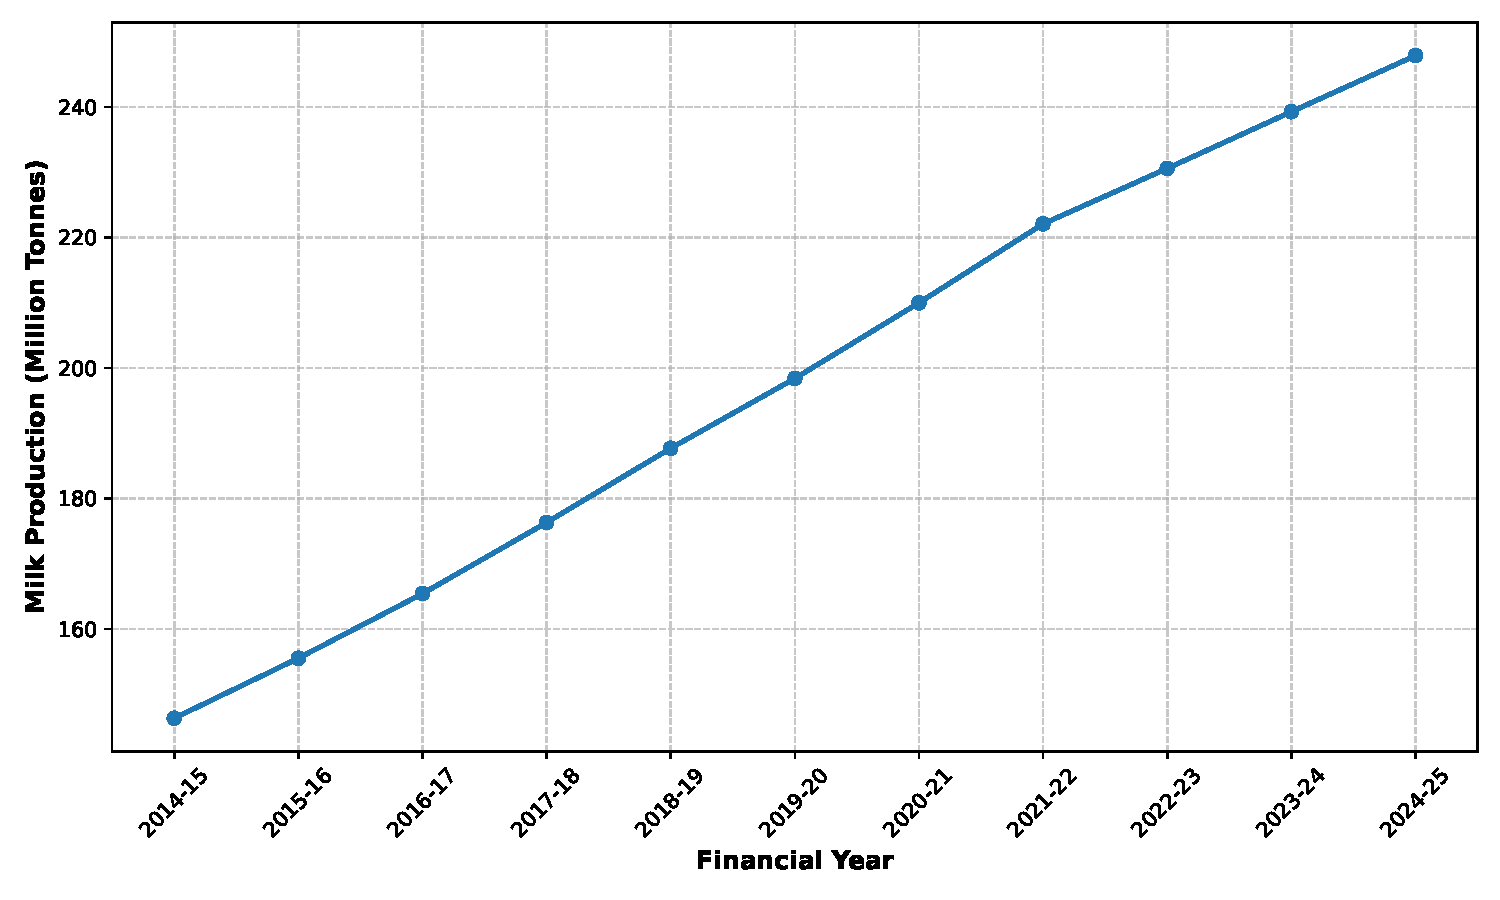
\includegraphics[width=0.72\textwidth]{milk_production_graph.pdf}
\caption{Growth of annual milk production in India from 2014--15 to 2024--25. Data compiled from the BAHS 2025 report \cite{pib2025bahs}.}
\label{fig:milk_growth}
\end{figure}

Milk's perishability imposes a rigid cold-chain requirement: transit from Village Collection Centres (VCCs) to processing plants must complete within a 4-hour window to keep microbial load within safety standards \cite{Shukla2013,Gupta2020}. In rural India this is compounded by road geometry. Following Ballou et al.\ \cite{BALLOU2002}, the average circuity factor for the Indian road network is approximately 1.31 (standard deviation 0.21), so actual travel distances commonly exceed straight-line distances by 30--50\% \cite{Giacomin2015}. When managing a heterogeneous fleet across hundreds of scattered collection points, manual route planning becomes computationally intractable and economically unjustifiable.

To address this, we propose an optimised routing system for the dairy network in the Buldhana and Nagpur regions of Maharashtra. The main contributions of this paper are three-fold:
\begin{itemize}
    \item \textbf{Real-World Road Geometry}: Integration of the Open Source Routing Machine (OSRM) with Google OR-Tools for a large-scale dairy MDVRP, mitigating the 30--50\% distance-estimation error inherent to Euclidean models \cite{BALLOU2002,Giacomin2015}.
    \item \textbf{Heterogeneous Fleet Optimisation}: A fleet model tailored to Indian rural constraints across 378 collection points, minimising total operational cost over homogeneous alternatives.
    \item \textbf{Strict Perishability Constraints}: Enforcement of a 4-hour maximum shift duration via time-dimension constraints and Guided Local Search (GLS) with node disjunctions, preserving solver feasibility while meeting safety windows.
\end{itemize}

\section{Related Work}
\label{sec_related}

The Vehicle Routing Problem (VRP) and its extensions---including the Capacitated VRP (CVRP), Time-Window VRPTW, Multi-Depot MDVRP, and Heterogeneous Fleet HFVRP---have been foundational to logistics optimisation. For large-scale instances like ours, exact solvers are computationally prohibitive. While Tabu Search and Simulated Annealing are popular, Guided Local Search (GLS) \cite{Voudouris1999} is particularly effective at escaping local optima on large instances by augmenting frequently traversed arcs with Lagrangian penalties. We thus utilise the GLS implementation in Google OR-Tools \cite{ORTools2024}.

Perishable goods routing extends standard VRP by introducing strict time-sensitive quality constraints to prevent non-linear microbial risk compounding. In the context of Indian dairy logistics \cite{Shukla2013,Gupta2020,NDDB2024}, prior studies have demonstrated route-length reductions via capacitated clustering \cite{Rautela2019}, sustainability models \cite{Patel2019}, and cost savings from heterogeneous fleets \cite{Ravichandran2020}. Most recently, Gheisariha et al.\ \cite{Gheisariha2023} scheduled heterogeneous vehicles for milk collection with time windows in a single-depot setting. We extend this foundation to a multi-depot configuration across 378 VCCs, uniquely integrating real-road geometry from OSRM---a geographic fidelity not previously reported.

\section{Methodology}
\label{sec2}

\subsection{Dataset and Study Area}
\label{subsec2}

The dataset was extracted from daily operational records of dairy cooperatives in the Buldhana and Nagpur regions of Maharashtra. Raw spreadsheet data were pre-processed and serialised into structured JSON for large-scale optimisation. The final dataset comprises 378 VCCs, each with a daily milk yield (litres) and geographic coordinates. The data were provided under a confidentiality agreement and cannot be publicly released; however, the pre-processing pipeline and solver code are available in the accompanying repository (\url{https://github.com/RAJ-A58/route_optmisation}).

Central to the network are six depots that serve as origin and destination for all vehicles, classified as Milk Collection Centres (MCC) or Bulk Milk Coolers (BMC) by their processing and cooling capability. The multi-depot configuration enables inter-depot optimisation so that each vehicle is dispatched from the facility that minimises overall travel cost. The MCCs are Buldhana ($20.9779^\circ$N, $76.1923^\circ$E), Buttibori ($20.9426^\circ$N, $78.9456^\circ$E), and Dhanoli ($21.0660^\circ$N, $78.6024^\circ$E); the BMCs are Manapur ($21.3825^\circ$N, $79.3228^\circ$E), Dahid ($20.4988^\circ$N, $76.0623^\circ$E), and Dhad ($20.3803^\circ$N, $75.9936^\circ$E).

\subsection{Heterogeneous Fleet and Cost Model}
\label{subsec2_2}

Real-world dairy logistics rarely justify a uniform fleet, given high variability in village yields. We therefore use a heterogeneous fleet of three categories, each defined by volumetric capacity, fixed daily activation cost, and variable cost per kilometre (Table~\ref{tab:fleet}). Cost parameters were derived from published manufacturer and freight-market benchmarks \cite{TataMotors2024,Eicher2024,Vahak2024}. To ensure sufficient availability without constraining the solution, a pool of 10 vehicles per type per depot was provided, yielding a global pool of 180 vehicles ($6\times3\times10$); the solver activates only the minimum number needed to minimise total cost.

\begin{table}[t]
\caption{Heterogeneous fleet specifications and operational costs \cite{TataMotors2024,Eicher2024,Vahak2024}}
\label{tab:fleet}
\centering
\small
\begin{tabular}{lccc}
\hline\noalign{\smallskip}
Vehicle Type & Capacity (L) & Fixed Cost (Rs.) & Cost/km (Rs.) \\
\noalign{\smallskip}\hline\noalign{\smallskip}
Heavy (10--12 Wheeler)   & 25{,}000 & 25{,}000 & 55 \\
Medium (6-Wheeler ICV)   & 7{,}000  & 15{,}000 & 28 \\
Light (SCV/Chhota Hathi) & 1{,}000  & 5{,}000  & 15 \\
\noalign{\smallskip}\hline
\end{tabular}
\end{table}

\subsection{Constraint Programming Model}
\label{subsec2_3}

The problem is formalised as a Constraint Programming model solved with the Google OR-Tools \texttt{RoutingModel} engine \cite{ORTools2024}. Let $V$ be the set of all nodes (depots and VCCs), $C\subset V$ the customer nodes, $K$ the vehicles, $d_{ij}$ the real-road distance (metres) between $i$ and $j$ from OSRM, $c_k$ and $f_k$ the variable per-km and fixed activation costs of vehicle $k$, $Q_k$ its capacity, and $q_i$ the demand at VCC $i$. Decision variables $x_{ijk}\in\{0,1\}$ denote arc traversal by vehicle $k$, $y_k\in\{0,1\}$ whether $k$ is activated, and $z_i\in\{0,1\}$ whether node $i$ is dropped via disjunction. The objective minimises variable travel cost, fixed activation cost, and disjunction penalties $P$:
\begin{equation}
\min\left[\sum_{k\in K}\sum_{i\in V}\sum_{j\in V} c_k\frac{d_{ij}}{1000}x_{ijk} + \sum_{k\in K} f_k y_k + \sum_{i\in C} P z_i\right]
\label{eq_obj}
\end{equation}
subject to: flow conservation, so each active vehicle departs from and returns to its depot $b(k)$,
\begin{equation}
\sum_{j\in V} x_{b(k),j,k} = \sum_{j\in V} x_{j,b(k),k} = y_k,\ \forall k\in K;
\label{eq_flow}
\end{equation}
customer visit, so each non-dropped customer is visited exactly once,
\begin{equation}
\sum_{k\in K}\sum_{j\in V} x_{ijk} = 1-z_i,\ \forall i\in C;
\label{eq_visit}
\end{equation}
capacity, so collected milk cannot exceed vehicle capacity,
\begin{equation}
\sum_{i\in C} q_i\sum_{j\in V} x_{ijk} \le Q_k y_k,\ \forall k\in K;
\label{eq_cap}
\end{equation}
shift duration, so every vehicle completes its route within the 4-hour window,
\begin{equation}
\tau^{k}_{b(k),\mathrm{ret}} - \tau^{k}_{b(k),\mathrm{start}} \le T_{\max}y_k;
\label{eq_time}
\end{equation}
and time propagation, so arrival times are consistent with travel durations,
\begin{equation}
\tau^{k}_{j} \ge \tau^{k}_{i} + \frac{d_{ij}}{v} + s_i,\ \forall(i,j)\in V^2,\ k\in K,
\label{eq_prop}
\end{equation}
where $T_{\max} = 14{,}400$~s is the maximum permitted shift duration (4 hours), $v=40$~km/h is the average rural transit speed, and $s_i$ the service time at node $i$.

A disjunction penalty $P=100{,}000$ (arc-cost units) is assigned to each customer node, allowing the solver to exclude a node only if its inclusion would violate \eqref{eq_time}; this guarantees a complete, valid solution rather than solver failure. The 40~km/h speed reflects rural road conditions and the high circuity factor ($\approx1.31$) of the Indian network \cite{BALLOU2002}. A 5-minute (300~s) pumping delay per VCC is included in the time-window model as a conceptual constraint for the mandatory milk transfer; the experiments in Sect.~\ref{sec3} use travel-time-only routing to isolate the geometric contribution of real-road distances, with service time recommended for production deployment. GLS \cite{Voudouris1999} is the primary improvement strategy, augmenting frequently traversed arcs with Lagrangian penalties to escape the premature convergence typical of standard local search on large MDVRP instances.

\subsection{Matrix Generation and Model Integration}
\label{subsec2_4}

Translating raw coordinates into a solvable model required a multi-stage pipeline. A duplicate-entry audit---stripping whitespace, upper-casing, and lexicographically sorting name tokens---merged redundant records and confirmed that the 378 VCCs are unique locations. Transit distances were obtained via OSRM \cite{Luxen2011} using its public routing API. Given the dataset scale, constructing the full $384\times384$ matrix required processing about 147{,}456 node pairs; to mitigate latency and rate limits, a chunked fetching algorithm (Algorithm~\ref{algo:mdvrp}) processed the node set in subsets of 50 with a 100~ms inter-request delay. The finalised matrix, vehicle cost structures, and node metadata were serialised into a JSON input for the OR-Tools engine.

\begin{algorithm}[t]
\caption{OSRM Chunked Matrix Construction and GLS Initialisation}
\label{algo:mdvrp}
\footnotesize
\begin{algorithmic}[1]
\Require Node set $V$ (384 nodes), Fleet $K$ (180 vehicles), Chunk size $B=50$
\Ensure Optimised multi-depot schedule $R$
\State $M\leftarrow\mathbf{0}$ \Comment{$|V|\times |V|$ distance matrix}
\For{each origin chunk $S_a\subseteq V$, destination chunk $S_b\subseteq V$ (size $B$)}
  \State Query OSRM Table API to retrieve real-road distances (m)
  \State $M[S_a][S_b]\leftarrow$ extracted distances
\EndFor
\State Initialise Constraint Programming routing model $\mathcal{M}$ over nodes $V$ and fleet $K$
\For{each vehicle $k\in K$}
  \State Define transit cost function $\lambda_k(i,j) \leftarrow \lfloor(M[i][j]/1000)\cdot c_k\rfloor$
  \State Register $\lambda_k$ and fixed activation cost $f_k$ to model $\mathcal{M}$
\EndFor
\State Enforce capacity ($Q_k$), maximum shift duration ($T_{\max}$), and disjunction penalties ($P$)
\State Configure heuristics: \texttt{PATH\_CHEAPEST\_ARC} (construction) and \texttt{GLS} (improvement)
\State $R\leftarrow$ Solve $\mathcal{M}$ within a 180~s computational limit
\end{algorithmic}
\end{algorithm}

\section{Results and Discussion}
\label{sec3}

The model was executed on the processed dataset to evaluate fleet efficiency, cost, and adherence to perishability constraints. The OSRM-integrated matrix lets the solver generate routes based on real road geometry rather than straight-line distances, directly addressing the 30--50\% circuity error \cite{BALLOU2002,Giacomin2015}.

\subsection{Cluster-Based Depot Performance}
\label{subsec3_1}

The engine partitioned the 378 VCCs into six geographic clusters under the 4-hour constraint (Table~\ref{tab:depot_performance}, Fig.~\ref{fig:depot_perf}). VCC-to-depot assignment is determined dynamically: each vehicle is dispatched from a specific depot, and the solver selects routes minimising the global objective \eqref{eq_obj}, implicitly assigning each VCC to whichever depot services it at lowest cost. This inter-depot optimisation reduces deadheading by returning vehicles to the most logically situated hub.

\begin{table}[t]
\caption{Operational summary by depot hub}
\label{tab:depot_performance}
\centering
\small
\begin{tabular}{lcccc}
\hline\noalign{\smallskip}
Depot & VCCs & Milk (L) & Fleet (H/M/L) & Veh. \\
\noalign{\smallskip}\hline\noalign{\smallskip}
BMC Dahid     & 29  & 4{,}725  & 0/0/5  & 5  \\
BMC Dhad      & 10  & 2{,}492  & 0/0/3  & 3  \\
BMC Manapur   & 67  & 25{,}855 & 0/3/6  & 9  \\
MCC Buldhana  & 51  & 6{,}616  & 0/0/7  & 7  \\
MCC Buttibori & 96  & 20{,}920 & 0/3/10 & 13 \\
MCC Dhanoli   & 124 & 23{,}373 & 0/5/10 & 15 \\
\noalign{\smallskip}\hline\noalign{\smallskip}
\textbf{Total} & \textbf{377} & \textbf{83{,}981} & \textbf{0/11/41} & \textbf{52} \\
\noalign{\smallskip}\hline
\end{tabular}
\end{table}

\begin{figure}[tb]
\centering
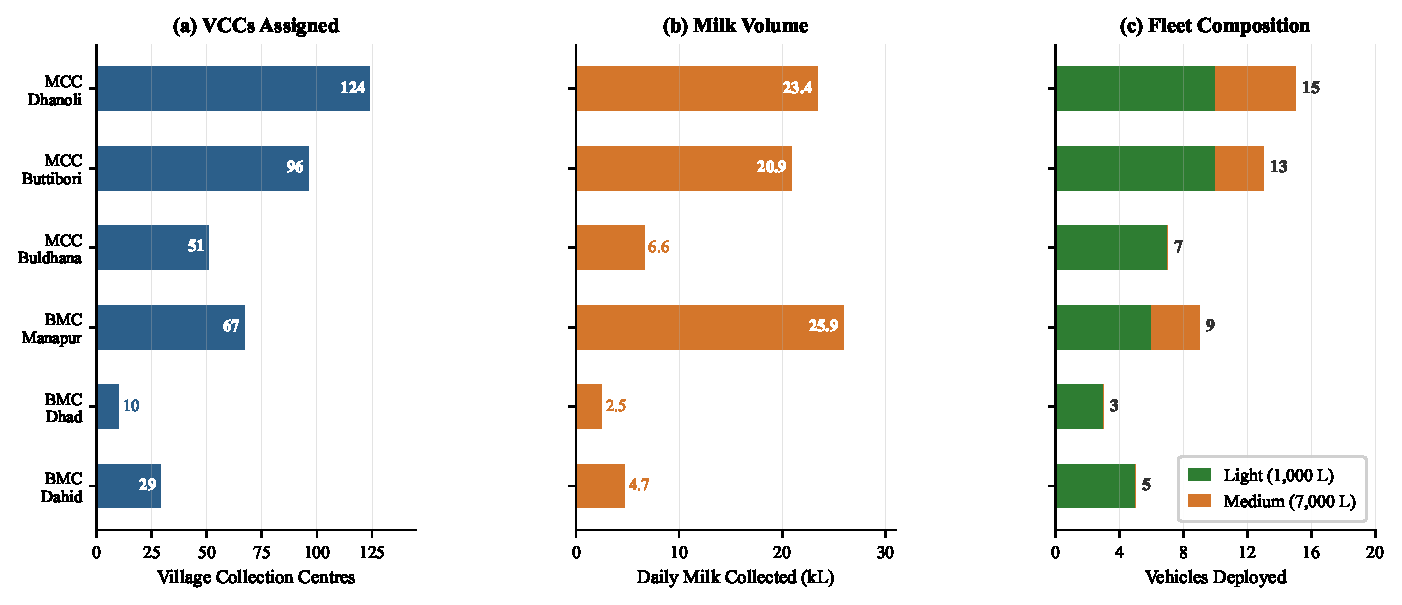
\includegraphics[width=0.72\textwidth]{figures/fig2_depot_performance.pdf}
\caption{Depot-level performance across the six hubs: (a) VCCs assigned, with MCC Dhanoli serving the largest cluster (124 VCCs); (b) daily milk yield collected per depot; (c) Light/Medium fleet composition---no Heavy tankers were activated at any depot.}
\label{fig:depot_perf}
\end{figure}

\subsection{Fleet Utilisation and Node Disjunctions}
\label{subsec3_2}

From the pool of 180 vehicles, the solver activated only \textbf{52 units} (41 Light, 11 Medium, 0 Heavy). Total network distance was \textbf{5{,}743.90~km} at an optimised cost of \textbf{Rs.~4{,}77{,}214.77}. No heavy tankers were deployed: rural road constraints and low-to-moderate per-village yields make light and medium vehicles strictly more cost-effective for this topology. The average route duration was about \textbf{3~h~17~min}, confirming that the 4-hour window is achievable for the overwhelming majority of centres at 40~km/h even after accounting for real-road circuity.

Under the 14{,}400~s shift limit and high rural circuity, \textbf{1 node}---Parsoda (156~L)---was excluded via disjunction, giving 99.7\% service coverage (377 of 378 VCCs). This exclusion provides a mathematically rigorous justification for cooperatives to investigate this zone as a candidate site for a new BMC or satellite chilling unit.

\subsection{Cost-Benefit and Algorithmic Benchmarking}
\label{subsec3_4}

Two homogeneous alternatives were evaluated with the same solver and OSRM matrix, varying only vehicle type (Table~\ref{tab:comparison}, Fig.~\ref{fig:cost_comparison}). The heterogeneous model achieves a daily cost reduction of \textbf{60.4\%} over a homogeneous heavy-tanker fleet and \textbf{31.4\%} over a homogeneous medium-truck fleet. These savings arise from two complementary effects: light vehicles incur much lower fixed and per-km costs on remote, low-yield villages, while medium trucks aggregate high-yield clusters without the excess-capacity penalty of heavy tankers.

\begin{table}[t]
\caption{Comparative cost-benefit benchmark}
\label{tab:comparison}
\centering
\small
\begin{tabular}{lccc}
\hline\noalign{\smallskip}
Configuration & Vehicles & Cost (Rs.) & Reduction \\
\noalign{\smallskip}\hline\noalign{\smallskip}
Homog.\ Heavy   & 38 & 12,01,117.13 & 60.4\% \\
Homog.\ Medium  & 38 & 6,96,055.80  & 31.4\% \\
\textbf{Heterogeneous} & \textbf{52} & \textbf{4,77,214.77} & \textbf{---} \\
\noalign{\smallskip}\hline
\end{tabular}
\end{table}

\begin{figure}[tb]
\centering
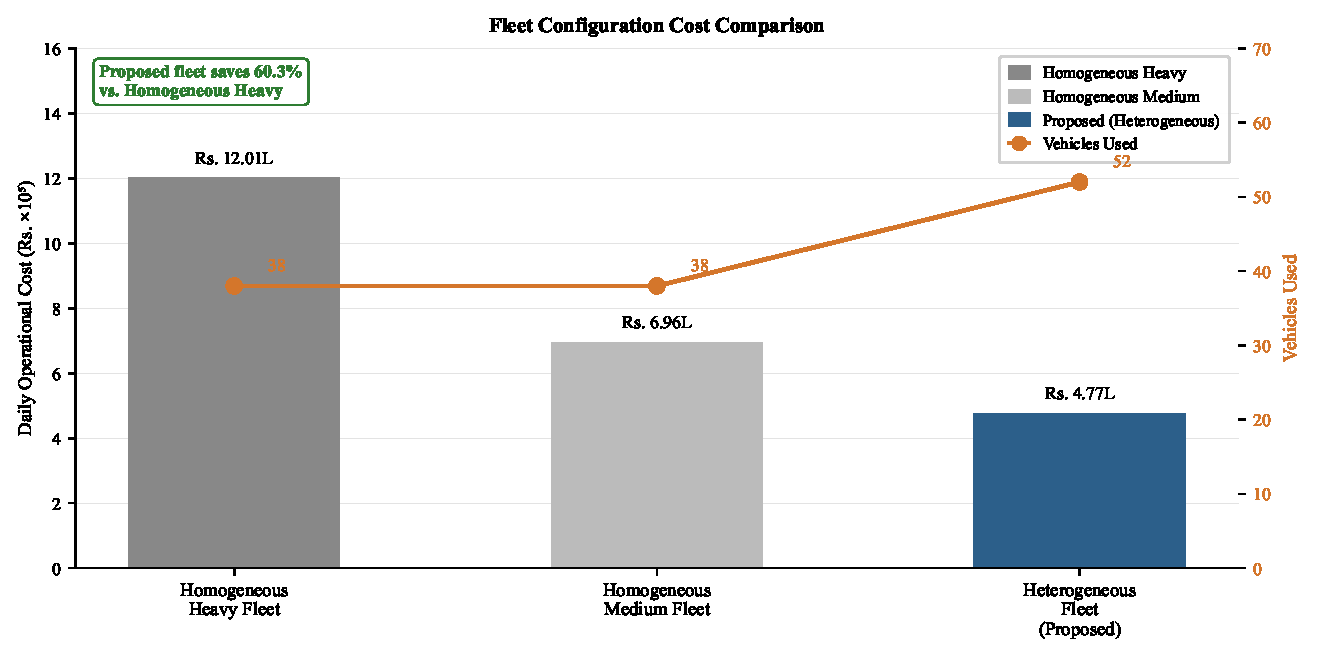
\includegraphics[width=0.72\textwidth]{figures/fig3_cost_comparison.pdf}
\caption{Fleet-configuration cost comparison. The proposed heterogeneous fleet cuts daily cost by 60.4\% versus homogeneous heavy tankers and 31.4\% versus homogeneous medium trucks, despite deploying more (smaller) vehicles.}
\label{fig:cost_comparison}
\end{figure}

To validate GLS for this topology, we benchmarked it against Tabu Search and Simulated Annealing, all initialised from the same first solution (\texttt{PATH\_CHEAPEST\_ARC}) under an identical 60~s wall-clock limit on the same instance and hardware (Fig.~\ref{fig:algo_bench}). GLS achieved the lowest total cost (Rs.~4,81,763.63 vs.\ Rs.~4,94,375.10 for the other two), deploying one fewer vehicle (51 vs.\ 52) by correctly identifying Parsoda as infeasible and excluding it---incurring the Rs.~1,00,000 penalty but saving more than that in detour cost. Tabu Search and Simulated Annealing converged to identical results because both start from the same deterministic solution and exhaust their neighbourhood within 60~s, confirming the known limitation of neighbourhood-based methods on large MDVRP instances and validating the penalty-augmentation strategy of GLS for this domain.

\begin{figure}[tb]
\centering
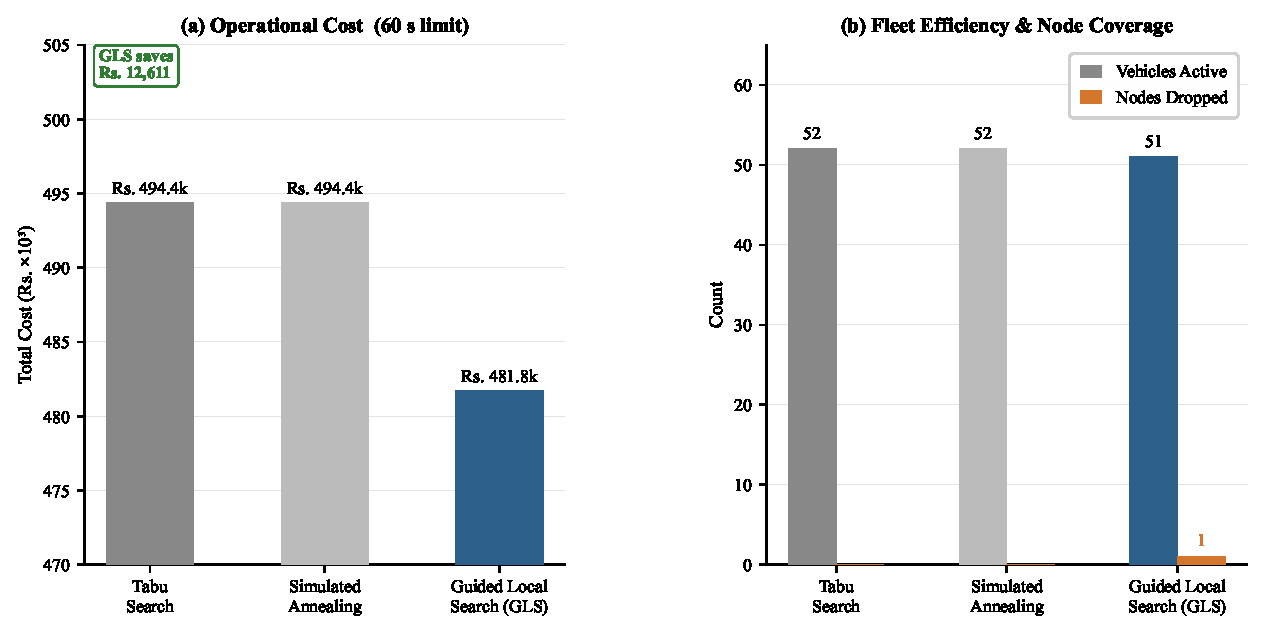
\includegraphics[width=0.72\textwidth]{figures/fig4_algorithm_benchmark.pdf}
\caption{Metaheuristic benchmark under a 60~s limit on an identical instance. (a) GLS attains the lowest cost, saving Rs.~12,611 over Tabu Search and Simulated Annealing. (b) GLS alone invokes the disjunction mechanism for Parsoda.}
\label{fig:algo_bench}
\end{figure}

\subsection{Sensitivity to Seasonal Yield}
\label{subsec3_6}

Indian dairy output is seasonal, with a high-yield ``Flush'' (winter) and a low-yield ``Lean'' (summer) period. Scaling all VCC demands by $\pm20\%$ and re-solving (Fig.~\ref{fig:sensitivity}) shows strong resilience: cost moves from Rs.~4,35,004.96 (Lean, 67{,}039~L, 46 vehicles) to Rs.~5,36,674.02 (Flush, 1,00,632~L, 53 vehicles), against the Rs.~4,77,214.77 base case (83{,}981~L, 52 vehicles). Rather than failing during the Flush season, the model scales Medium-truck use from 11 to 16 units to absorb the additional 16{,}651~L, while Light trucks adjust downward to avoid unnecessary fixed-cost activation. Cost scales near-linearly with volume, and the number of dropped nodes remains constant at 1 across all scenarios, confirming stable solver behaviour under demand perturbation.

\begin{figure}[H]
\centering
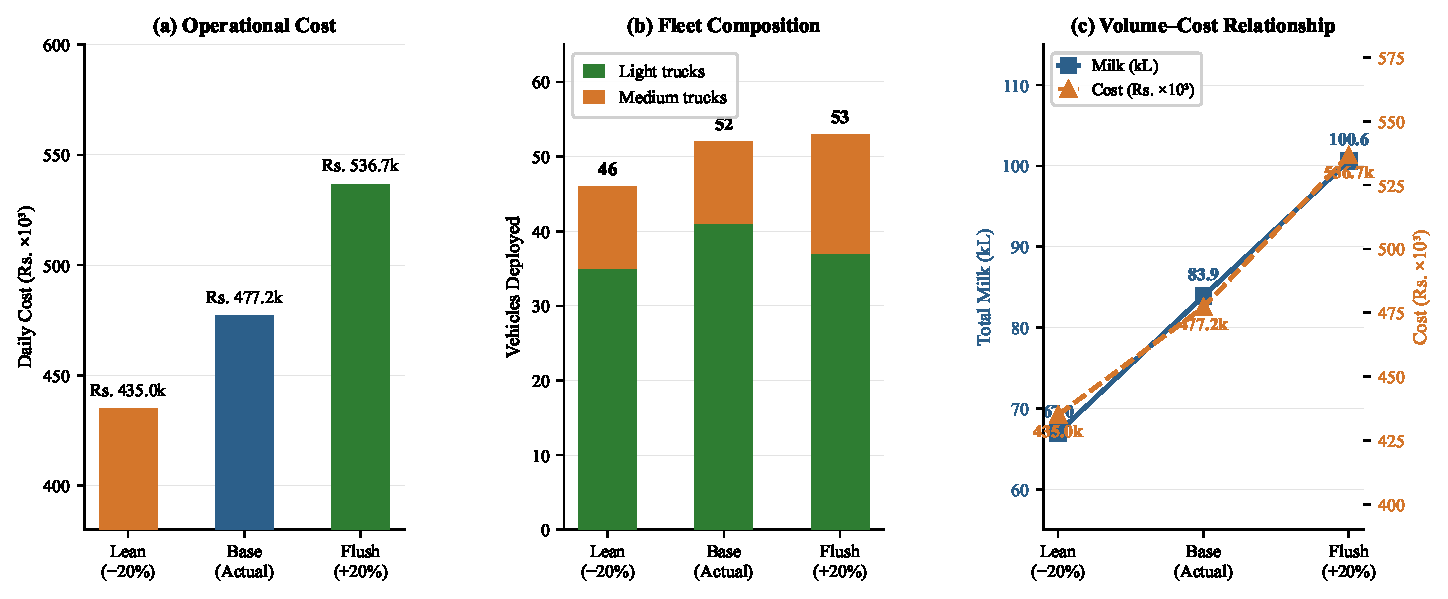
\includegraphics[width=0.72\textwidth]{figures/fig5_seasonal_sensitivity.pdf}
\caption{Seasonal demand sensitivity ($\pm20\%$). (a) Cost rises near-linearly from Rs.~4,35,004.96 (Lean) to Rs.~5,36,674.02 (Flush). (b) Medium-truck use rises from 11 to 16 units in the Flush season while Light trucks adjust downward. (c) The volume--cost relationship is near-linear; dropped nodes stay constant at 1.}
\label{fig:sensitivity}
\end{figure}

\section{Conclusion}
\label{sec4}

This work presents an operational Constraint Programming solution for the Capacitated Multi-Depot Vehicle Routing Problem with Time Windows tailored to Indian cooperative dairy networks. Integrating real-road distances from OSRM with OR-Tools Guided Local Search directly addresses the 30--50\% Euclidean circuity distortion prevalent in Indian rural roads. On operational data for 378 VCCs and 6 depots across Buldhana and Nagpur, the solver achieved 99.7\% service coverage (377/378 VCCs), activating 52 vehicles at Rs.~4,77,214.77/day---31.4\% below conventional medium trucks and 60.4\% below heavy tankers. The isolated Parsoda node offers a data-driven basis for a new BMC, and the seasonal analysis shows the model scales gracefully across $\pm20\%$ demand without compromising safety. Future work will add stochastic demand forecasting, real-time traffic, and multi-objective cost--emissions--equity optimisation.

\section*{Acknowledgments}
The authors used Claude (Anthropic) to assist with restructuring, condensing, and formatting the manuscript into the SoCTA LaTeX template. All technical content, results, and analysis are the authors' own.

\bibliographystyle{spmpsci}
\bibliography{references}

\end{document}
